\documentclass[report]{../../custom}
\begin{document}
\maketitle

\noindent \textbf{摘要:}

\vskip 0.5cm

\noindent \textbf{下周计划:} 1)GPU并行化实现FORS和HT树,2)推进论文写作。

\section{论文阅读}

本周主要阅读了 \cite{Wang2025},该文对于如何并行化实现SPHINCS+签名算法进行了深入的研究。其中对签名中的HT树、FORS树、WOTS+算法进行了并行化实现,并依据其各组件先后运行的顺序,对其进行分层并行,从上到下一共进行了4层的并行化。由于分层后,各层之间的相互独立,因此\cite{Wang2025}中可以对各层之间的并行化进行组合,依据具体的资源情况进行选择,从而实现\textcolor{blue}{更高的并行效率(PE)},i.e. PE=效率/资源。

这种组合方式下能够获得更高的PE,但是为能获取到最优的PE,因此获取一个最优的PE为我们创新方向。具体展开来说,以图 \ref{fig:merkle_tree_paralle} 为例,左侧为最大并行化的情况,其将每次HASH运算作为一个任务,同时导致需要四次同步操作,为此导致计算的不平衡性,使计算之间出现等待。而右侧则是最小并行化的情况,其将所有HASH运算作为二个任务,减少计算之间的不平衡性,但是其并行度较低。因此我们计划在这两种策略之间,寻取一个\textcolor{blue}{中间HASH运算的分组数},使得计算之间的不平衡性和并行度达到一个平衡,从而获得更好的PE。

\begin{figure}[!ht]
  \centering
  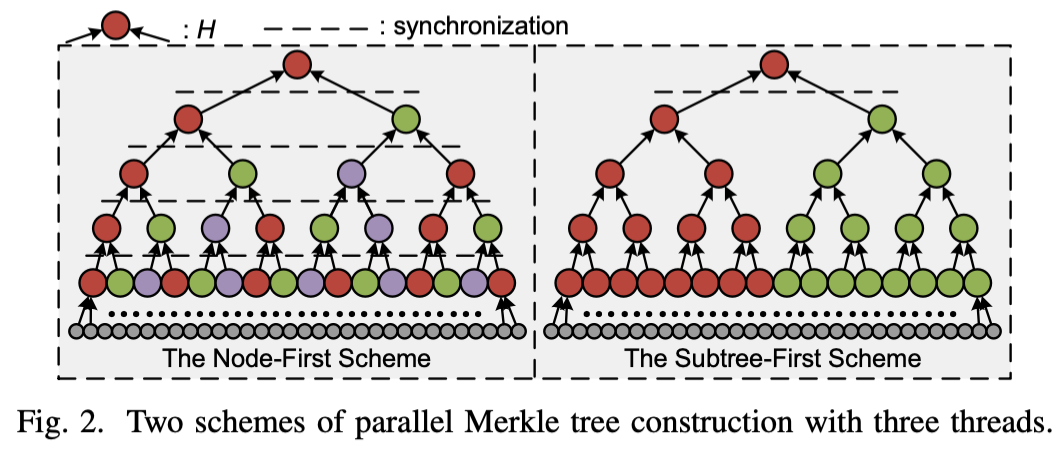
\includegraphics[width=0.6\textwidth]{./fig/merkle_tree_paralle.png}
  \caption{Merkle Tree 并行化\cite{Wang2025}}
  \label{fig:merkle_tree_paralle}
\end{figure}

\bibliographystyle{alpha}
\bibliography{../../paper}

\end{document}